\section{引言}

\subsection{自主反应机理研究的物理要求}

有机反应机理的科学有效性检验，需要核对每个物种和基元步骤所对应的分子几何、反应路径与量子化学结果。几何优化正常终止（exit 0）说明计算程序已完成运行。判断所得结构是否为稳定中间体，还需通过频率计算确认极小值；为一阶鞍点指定反应步骤，则需通过 IRC 确定两侧连接的物种。IRC 若到达另一个解离产物或立体异构体，相应能量计算的机理归属也随之改变。包含多个基元步骤或竞争立体路径的研究，需要逐一确定每个鞍点连接的物种。\citep{ref09,ref10}

计算化学智能体已能自动执行其中的若干环节。El Agente Q \citep{ref01}、Aitomia \citep{ref02} 与 Gráfico \citep{ref06} 编排量子化学计算及类型化工作流；Estructural \citep{ref04} 与 ARCHE \citep{ref05} 提供分子片段编辑、原子映射及过渡态几何准备工具；Quntur \citep{ref03} 研究反应动力学与过渡态。将这些能力推进到自主机理探索，还需要可靠的几何操作，以及对计算所得物种和路径的物理解释。

立体取向对齐、反应片段装配与路径端点准备都涉及三维几何关系。语言模型在直接推断这些关系或操作笛卡尔坐标时可能出错。例如，Quntur \citep{ref03} 报告复杂路径与过渡态准备需要人工协助端点对齐。模型可让程序绕指定化学键旋转一侧原子，再测量相关二面角，据此比较和选择过渡态初猜。

候选中间体必须优化为极小值；候选过渡态必须是一阶鞍点，且其路径连接目标反应物和产物。若 IRC 通向另一产物或立体异构体，该鞍点应归入其实际连接的反应。自主探索系统需要据此重新判断步骤归属，或继续寻找目标鞍点。

\subsection{Cloudra：以化学对象组织自主机理探索}

以工具调用或计算任务为节点、执行依赖为边的工作流图，规定计算如何组织。Cloudra 是面向有机小分子机理探索的多智能体系统，要求智能体用 Delivery DAG 中的物种对象和基元反应步对象表达交付机理。智能体根据当前的结构和能量提出假设，选择要探索的步骤和下一项计算。

图~\ref{fig:01}展示85个化学 AI Agent 系统的结构化文献样本：材料或表面39项，有限分子或配合物23项，软物质或生物分子12项，另有11项展示多个对象类别。图~\ref{fig:02}和图~\ref{fig:03}展示有限分子或配合物类已记录的任务，并对比 Cloudra 与已有系统的能力覆盖。配套文献材料保留完整矩阵及逐项来源。

\begin{figure}[tbp]
\centering
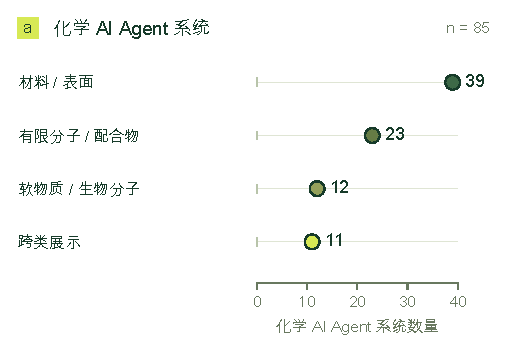
\includegraphics[width=\linewidth]{figures/fig01.pdf}
\caption{85个化学 AI Agent 系统的结构化文献样本：材料/表面39项、有限分子/配合物23项、软物质/生物分子12项、跨类系统11项。}
\label{fig:01}
\end{figure}

按照“智能克制”的原则，Cloudra 将坐标计算交给确定性程序。MCS 匹配用于选择分子片段，原子映射用于匹配反应物与产物中的原子，并标出成键或断键的原子对。程序测量键长、键角、二面角与立体特征，并通过旋转或平移选定原子来构造候选结构。

\begin{figure}[tbp]
\centering
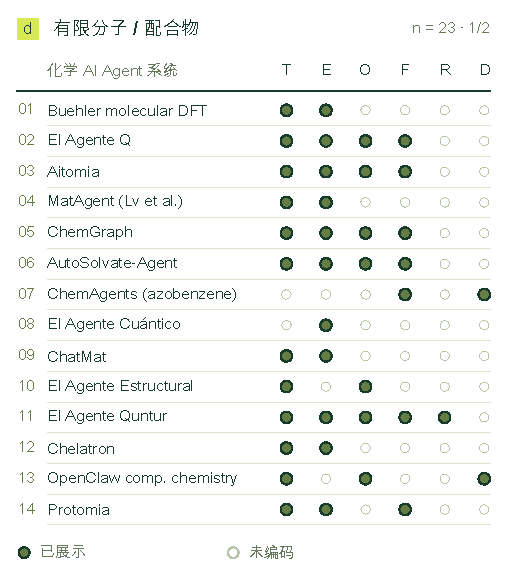
\includegraphics[width=\linewidth]{figures/fig02.pdf}
\caption{有限分子/配合物类已记录的任务（第1/2面板，共23个化学 AI Agent 系统）。T：结构构建/编辑；E：静态能量/性质；O：几何优化；F：振动/热化学；R：显式路径/过渡态；D：分子/量子动力学。实心表示文献提供正面证据，空白项的能力覆盖保留为未知。}
\label{fig:02}
\end{figure}

Delivery DAG 将机理表示为化学对象组成的图。每个物种节点承载分子几何、成键拓扑、立体构型及相应计算结果；每条基元反应步的边承载过渡态和连接相邻物种的反应路径。分子拓扑与立体化学比较确定物种身份，原子映射确定反应物与产物中的原子对应关系。频率计算判定驻点性质，IRC 端点计算确定其反应连接。程序检查频率计算和双向 IRC 是否对应同一一阶鞍点，以及两侧末帧优化后是否得到声明的反应物和产物。Supervisor 对照题目审阅这些对象，并指出还需完成的计算和还需研究的步骤。

\begin{figure}[tbp]
\centering
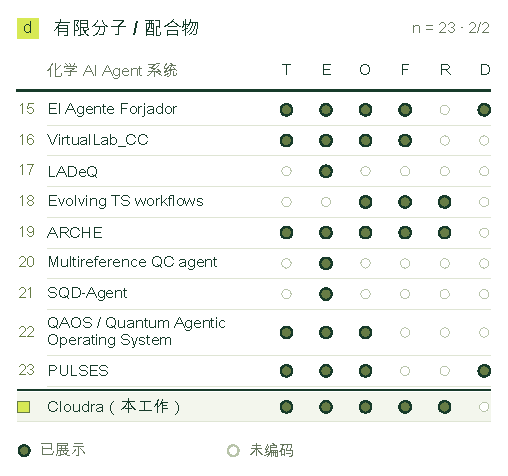
\includegraphics[width=\linewidth]{figures/fig03.pdf}
\caption{有限分子/配合物类化学 AI Agent 系统任务续图（第2/2面板），代码同图~\ref{fig:02}，底端展示 Cloudra（本工作）的能力覆盖。全部85个化学 AI Agent 系统的完整矩阵及逐项来源限制见配套材料。}
\label{fig:03}
\end{figure}

\subsection{主要贡献}

Cloudra 的核心设计是将交付机理的图约束，与建立和操作化学对象的化学信息学算法结合起来。分子拓扑与立体构型标识物种，原子映射确定结构间的原子对应关系；几何操作构造候选结构，频率和 IRC 计算确定所得驻点及其反应连接。智能体围绕这些对象扩展和修订机理。

几何程序包括基于 MCS 的片段选择、用于确定移动原子组的图遍历，以及过渡态片段装配。智能体可旋转选定基团、调整片段位置、测量所得结构，并在过渡态搜索失败后准备新的初猜。

CloudraBench 用于衡量这套方法的端到端机理计算能力，依据原生计算产物评价图结构覆盖、物理自洽性和任务规定目标的准确度。50题涵盖基元与多步反应、立体化学及允许方法的适用边界。实验包括四题三次重复的48次运行，以及覆盖50题、四种配置的200次全基准运行。主要比较采用同一模型主干的 Standard，Record 与 Brief-errors 分析证据组织和诊断反馈的作用。
